\chapter{Revisão Bibliográfica}
% Label para referenciar
\label{revisao}
Este estudo tem como intuito a criação de uma plataforma que auxilie a população no combate a desinformação e contribua com o processo democrático brasileiro. Para este fim, tecnologias emergentes do cenário tecnológico foram utilizadas visando um processamento massivo de dados que se caracterizam por sua heterogeneidade. Logo, neste capítulo, os conceitos pertinentes relacionados às características de uma democracia serão discutidos, além do embasamento tecnológico necessário para prover o entendimento deste projeto.

\section{Democracia} Pode-se observar a existência de dois tipos de democracia ao redor do globo. A Democracia Direta, também conhecida como Democracia Pura, na qual todos os cidadãos detêm o poder de participar diretamente do processo de tomada de decisão. Os modelos atuais adotaram a Democracia Representativa, na qual indivíduos são eleitos para representar os interesses de determinado grupo no processo de tomada de decisão do Estado \cite{impactofictonreiforcingcitizens}. 

Alguns autores defendem que a Democracia Direta seria mais adequada em uma sociedade democrática considerando a efetividade de sua participação nos processos decisórios, porém este modelo apresenta uma impossibilidade técnica devido às barreiras de comunicação existentes, fator esse que pode ser reavaliado conforme a tecnologia vem tornando-se cada vez mais presente em nossa sociedade \cite{impactofictonreiforcingcitizens}.

\subsection{Democracia Digital} Com a chegada da internet, uma discussão que entra em pauta é a participação política da esfera civil, algo inimaginável anteriormente, mas que se torna plausível com os meios de comunicação disponibilizados pela tecnologia \cite{democraciadigital}.

Esse novo modelo de política parte do pressuposto que o cenário político está em crise e que a esfera pública não representa a esfera civil adequadamente, uma vez que o único vínculo constitucional existente dos atores públicos com a esfera civil é de natureza eleitoral, onde os civis não possuem qualquer tipo de influência nas decisões tomadas pelo Estado \cite{democraciadigital}.

Esse cenário nos faz questionar sobre a legitimidade da Democracia Representativa e uma nova experiência democrática possibilitada pelas tecnologias de redes de computadores entra em questão. Este modelo é caracterizado pela participação da esfera civil na política de maneira ágil e conveniente, sem a necessidade de entidades intermediárias. Esse novo modelo permite que a população não seja apenas consumidora das informações políticas, mas capaz de ser uma produtora e que consuma suas próprias informações para a sua intervenção na tomada de decisão política. Além disso, a Democracia Digital apresenta diversos graus para definir a influência da esfera civil no processo decisório, um deles 
é constituído por um Estado que consulta a sua população através de portais eletrônicos com o intuito de analisar as opiniões dos civis a respeito dos temas da agenda pública \cite{democraciadigital}.

\section{Computação em Nuvem} Computação em Nuvem, ou \textit{Cloud Computing}, define uma modalidade de computação que se diferencia pela disponibilização de recursos computacionais, sendo esses recursos infraestrutura, plataforma, \textit{software}, serviço ou armazenamento, de maneira dinâmica e escalável sob demanda \cite{cloudcomputing}. 

Trata-se de um ambiente compartilhado entre vários usuários onde o custo desses recursos segue a lógica de \textit{pay as you go}, ou seja, o usuário é cobrado pelo tempo de utilização de determinado recurso na plataforma de \textit{Cloud}. O fator crucial que permitiu aos provedores de nuvem o gerenciamento e segurança desse ambiente é a virtualização, uma vez que torna-se possível o isolamento de aplicações sendo executadas no mesmo \textit{hardware} \cite{cloudcomputing}.

\section{Big Data} O termo Big Data teve sua primeira aparição como uma tecnologia emergente em 2011 pelo Gartner, em sua análise denominada \textit{Hype Cycle for Emerging Technologies}, que identifica novas tendências no cenário tecnológico mundial, além de reconhecer o ponto em que se encontra \cite{bigdataincontext}.

O \textit{Hype Cycle} do Gartner foi introduzido em 1995 com o intuito de descrever o progresso das tecnologias emergentes no mercado através de uma curva, denominada como \textit{Hype Curve} \cite{understandinghypecicles}.

% Figura
\begin{figure}[H]
	\centering	
	\caption[\hspace{0.1cm}Fases do \textit{Hype Cycle}]{Fases do \textit{Hype Cycle}}
	  \vspace{-0.4cm}
	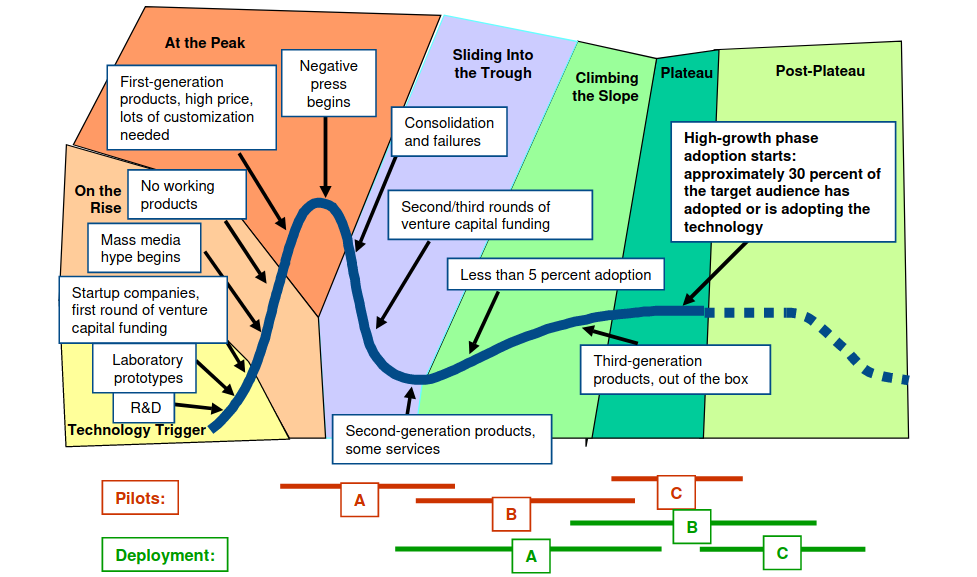
\includegraphics[width=.8\textwidth]{TCC/figuras/explaining_hype_cycle.png}
	% Caption centralizada
 	\captionsetup{justification=centering}
	% Caption e fonte
	 \vspace{-0.3cm}
	\\\textbf{\footnotesize Fonte: Gartner Research}
	\label{fig:tela1}
\end{figure}

A figura 1 demonstra as fases do ciclo, e elas são detalhadas abaixo:

\begin{itemize}
\item \textbf{\textit{Technology Trigger}}: Demonstração de protótipos e pesquisas em laboratório que provocam interesse do público e da indústria;
\item \textbf{\textit{On the Rise}}: Caracterizada pelas expectativas infladas, essa fase é marcada pelo impacto potencial que essa tecnologia terá no mercado e na sociedade como um todo. Primeiras gerações de produtos que demonstram pouca usabilidade, alta especificidade e custos altos de produção/implementação;
\item \textbf{\textit{At the Peak of Inflated Expectations}}: Após a disponibilização da primeira geração dos produtos, a tecnologia é levada aos seus limites conforme a distribuição e o uso são ampliados. As empresas começam a analisar a viabilidade e o benefício de aderir a tecnologia;
\item \textbf{\textit{Sliding Into the Trough of Disillusionment}}: O vale da desilusão ocorre quando a tecnologia falha ao buscar atender as expectativas infladas criadas pela mídia e é desacreditada. Nessa etapa, os produtos são melhorados com os \textit{feedbacks} dos clientes e tenta-se destacar os benefícios da adoção dessa tecnologia;
\item \textbf{\textit{Climbing the Slope of Enlightenment}}: Experiências reais e experimentações aumentam em diversos segmentos, levando à um melhor entendimento da tecnologia. Novas gerações de produtos são desenvolvidas e empresas mais flexíveis e tecnologicamente agressivas passam a adotá-la;
\item \textbf{\textit{Entering the Plateau of Productivity}}: Essa fase significa a entrada da tecnologia para a adoção do público \textit{mainstream}, onde os benefícios da tecnologia já são publicamente reconhecidos. Usualmente essas tecnologias são absorvidas em ecossistemas tecnológicos que ampliam sua adoção e sua maturidade; 
\item \textbf{\textit{Post-Plateau}}: Nesta fase a tecnologia já passou por todas as etapas e já se consolidou como parte do cenário tecnológico.
\end{itemize}

Como pode-se observar na figura 2, em 2011, o termo Big Data estava na fase \textit{On the Rise}, se caracterizando por uma alta expectativa relacionada ao seu possível impacto no mercado. Na última análise disponibilizada pelo Gartner, em 2019, a tecnologia não está presente no gráfico, uma vez que, atualmente, está na fase \textit{Post-Plateau} onde já se consolidou e já é uma realidade no mercado\footnote{Disponível em <https://www.gartner.com/smarterwithgartner/5-trends-appear-on-the-gartner-hype-cycle-for-emerging-technologies-2019/> Acesso em: 31 mai, 2020}.

% Figura
\begin{figure}[H]
	\centering	
	\caption[\hspace{0.1cm}\textit{Big Data} no \textit{Hype Cycle}]{\textit{Big Data} no \textit{Hype Cycle}}
	  \vspace{-0.4cm}
	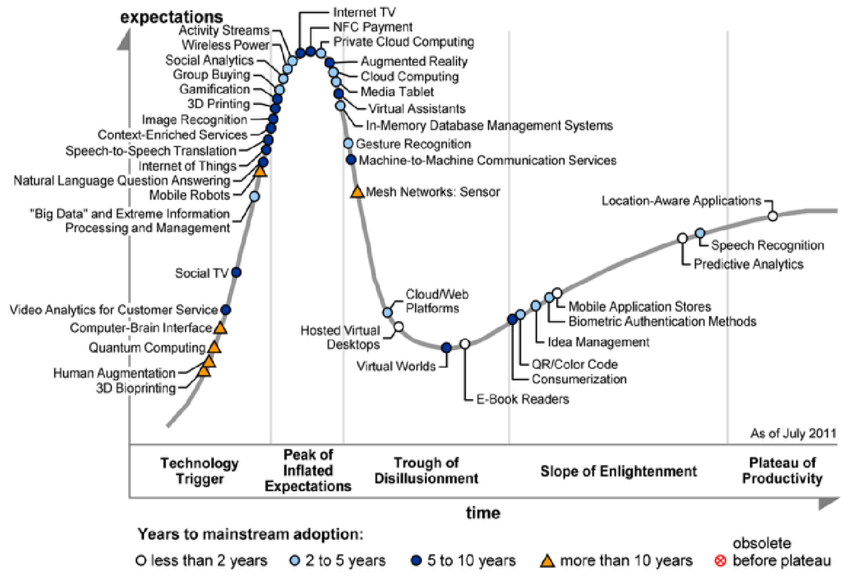
\includegraphics[width=.8\textwidth]{TCC/figuras/Hype-Cycle-for-emerging-technologies-Source-Gartner-Group-2011.png}
	% Caption centralizada
% 	\captionsetup{justification=centering}
	% Caption e fonte
	 \vspace{-0.3cm}
	\\\textbf{\footnotesize Fonte: Gartner (2011)}
	\label{fig:tela1}
\end{figure}

Big Data pode ser definido como um cenário onde existe uma volumetria massiva de dados com expressiva heterogeneidade de tal forma que seu processamento se torna inviável utilizando os métodos e tecnologias tradicionais. Dados estruturados, semi-estruturados e não estruturados precisam ser extraídos e analisados, porém essa complexidade torna impossível o gerenciamento e processamento nos moldes tradicionais. Para este ambiente, temos 3 pontos basilares deste conceito emergente, também comumente conhecidos como os 3 V's de Big Data \cite{bigdatafastdatadatalake}. São eles:
\begin{itemize} 
 \item \textbf{Volume}: Trata-se de uma volumetria massiva de dados; 
 \item \textbf{Variedade}: Dados caracterizados por sua heterogeneidade, sendo eles estruturados, semi-estruturados e não estruturados;
 \item \textbf{Velocidade}: Altíssima velocidade em que os dados são gerados e processados.
\end{itemize}

\section{\textit{Extract, Transform and Load (ETL)}} Um sistema ou processo de \ac{ETL} pode ser considerado como tudo entre a origem do dado e a camada de apresentação do seu sistema analítico. Consiste em três etapas:
\begin{itemize}
\item \textbf{\textit{Extract}}: A extração é o primeiro passo de um processo de ETL. É a etapa onde os dados necessários para análise precisam ser extraídos dos sistemas de origem e inseridos no ambiente analítico para as manipulações necessárias;
\item \textbf{\textit{Transform}}: Uma vez que o dado já está no ambiente analítico e pode ser facilmente analisado, inicia-se a etapa de transformação, que consiste em corrigir e normalizar o dado (tipagem, valores nulos, conflitos de domínio), além de relacionar múltiplas fontes de dados para agregar o valor máximo para o negócio;
\item \textbf{\textit{Load}}: A última etapa do processo é caracterizada pela carga ou inserção dos dados processados na etapa de transformação em um ambiente analítico.
\end{itemize}
Ao final deste processo , as bases de dados está atualizada e é disponibilizada para ferramentas de análise e visualização que fornecem os resultados com as partes interessadas \cite{thedatawarehousetoolkit}.

\section{Data Lake} Se tratando do conceito de Data Lake, sua estrutura é flexível. O Data Lake pode ser definido como um repositório massivo, centralizado e escalável de dados, contendo dados em seu formato de origem, além de possibilitar sua ingestão e processamento neste ambiente \cite{bigdatafastdatadatalake}. 

Uma particularidade do Data Lake é a separação do processamento e do armazenamento. Quando comparado com o Data Warehouse, por exemplo, um servidor ou mesmo um \textit{cluster} de servidores possuem a unidade de processamento e de armazenamento nos mesmos nós. Ou seja, uma instância é responsável pela execução das consultas aplicadas a ele e também do armazenamento dos dados propriamente ditos. Com a ascensão das tecnologias de Computação em Nuvem, temos o barateamento dos serviços de armazenamento, fator essencial para a construção de um Data Lake, onde temos um \textit{storage} escalável e o processamento é realizado a parte, onde utiliza-se de computação distribuída sob demanda \cite{datalakeforenterprises}. 

O Data Lake é segmentado em zonas, baseado nas condições e nos objetivos dos dados, conforme descrito abaixo:

\begin{itemize}
 \item \textbf{\textit{Raw Zone}}: É a zona onde os dados são importados. Nesta zona, os dados não sofrem alteração alguma e o seu formato é exatamente igual ao disponibilizado pelo sistema de origem; 
 \item \textbf{\textit{Staged Zone}}: Os dados já sofrem transformações com o intuito de padronização. Transformações como de/paras, transformação de \textit{encoding}, formatos de data, entre outras. Operações que tem o único objetivo de manter todos os dados na mesma estrutura para análises posteriores;
 \item \textbf{\textit{Curated Zone}}: Os dados já estão completamente tratados e prontos para as análises dos usuários de negócio. Inclusive os resultados de análises que são disponibilizados aos usuários e \textit{stakeholders}.
 \end{itemize}
 
 Essa separação em zonas torna o ambiente analítico mais flexível, o que possibilita que os Cientistas de Dados apliquem seus modelos de aprendizado de máquina nas zonas onde a granularidade dos dados é menor, por exemplo a \textit{Staged Zone}, enquanto os indicadores de negócio podem ser gerados a partir dos dados curados e prontos para análise na \textit{Curated Zone} \cite{datalakeforenterprises}.

\section{Apache Spark} O Apache Spark pode ser definido como uma plataforma computacional de alta velocidade e de propósito geral utilizada para o processamento distribuído de grandes massas de dados. Foi criado em 2009 na UC Berkeley e, posteriormente, passou a fazer parte da Apache Foundation\footnote{Disponível em <https://databricks.com/spark/about> Acesso em: 01 jun, 2020}. Para este trabalho, o processamento foi realizado principalmente utilizando esta plataforma, logo, a explicação do seu funcionamento se torna pertinente. Contém módulos com objetivos específicos, como descrito na figura 3, sendo eles \cite{learningspark}:

% Figura
\begin{figure}[H]
	\centering	
	\caption[\hspace{0.1cm} Spark]{Arquitetura Spark}
	  \vspace{-0.4cm}
	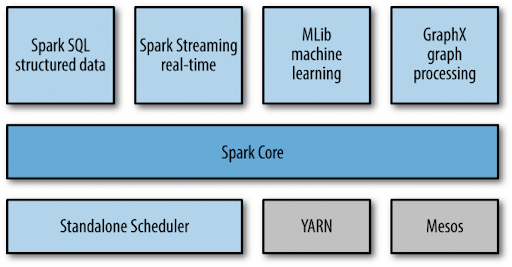
\includegraphics[width=.8\textwidth]{TCC/figuras/spark.png}
	% Caption centralizada
% 	\captionsetup{justification=centering}
	% Caption e fonte
	 \vspace{-0.3cm}
	\\\textbf{\footnotesize Fonte: Apache}
	\label{fig:tela1}
\end{figure}

\begin{itemize}
 \item \textbf{\textit{Spark Core}}: Spark Core contém toda a estrutura para o funcionamento do Spark. Os componentes para armazenamento, gerenciamento de memória, agendamento de tarefas, aém de definir as o conceito dos \textit{Resilient Distributed Datasets} (RDDs), o conceito basilar da plataforma; 
 \item \textbf{\textit{Spark SQL structured data}}: Spark SQL é o pacote utilizado para prover a manipulação de dados estruturados. Trabalha com diversas fontes de dados incluindo JSON, CSV, SQL, Parquet, entre outras. Possibilita ao usuário utilizar uma sintaxe SQL para manipulação dos dados, além do conceito dos \textit{Dataframes}, que podem ser definidos como um RDD com \textit{schema} e funcionalidades similares ao SQL;
 \item \textbf{\textit{Spark Streaming real-time}}: Spark Streaming é o módulo do Apache Spark capaz de processar dados em \textit{streaming}. Ele é capaz de realizar esse processamento através de micro processos em \textit{batch};
 \item \textbf{\textit{MLib machine learning}}: Pacote que fornece diversas APIs aos usuários para trabalhar com métodos estatísticos e algoritmos de \textit{Machine Learning}. Possui funções prontas de algoritmos de classificação, regressão, clusterização, entre outros. Estes métodos se beneficiam da computação distribuída do Spark Core para realizar o processamento;
 \item \textbf{\textit{GraphX graph processing}}: APIs para manipulação de grafos, além de possibilitar a computação distribuídas dessas estruturas de dados, uma vez que utilizam a implementação do Spark Core.
 \end{itemize}
 
O Spark possui recursos para gerenciar de maneira eficiente e escalabidade dos seus processos, distribuindo o processamento de um único nó a milhares de nós. O componente responsável por esse gerenciamento é o \textit{cluster manager}. O Apache Spark suporta três opções de \textit{managers}, sendo eles o Hadoop YARN, o Apache Mesos e o \textit{cluster manager} disponibilizado dentro do próprio Spark denominado Standalone Scheduler \cite{learningspark}.
 
\subsection{\textit{Resilient Distributed Datasets (RDDs)}}
Uma das abstrações principais do Spark Core é o conceito dos \textit{Resilient Distributed Datasets} (RDDs), que por sua vez podem ser definidos como coleções imutáveis e distribuídas de objetos. São separados em partições que possibilitam o processamento distribuído através do \textit{cluster}. Os RDDs possuem dois tipos de operações, sendo eles as \textit{transformations} e as \textit{actions}. Suas operações são baseadas em um conceito da computação denominado \textit{Lazy Evaluation}, que significa que as \textit{transformations}, operações que transformam o dado como métodos \textit{map} ou \textit{filter}, não serão executadas no momento em que são invocadas, mas sim empilhadas e organizadas em um grafo acíclico dirigido de instruções que serão aplicadas aos dados quando uma \textit{action}, operação de saída, como uma escrita no \textit{shell} ou em um arquivo, for disparada \cite{learningspark}.

\section{Trabalhos Relacionados}
\label{Trabalhos Relacionados}
Nos últimos anos, houveram inúmeros projetos que tratam e analisam dados
públicos com o intuito de informar a população brasileira, partindo tanto da esfera pública como da própria sociedade civil. 

Um dos projetos que trouxe grande engajamento por parte da comunidade para a análise de dados políticos foi o projeto Serenata de Amor que, através do uso de aprendizado de máquina, analisa os reembolsos realizados pela Câmara dos Deputados divulgados em sua plataforma de Dados Abertos, identificando atividades incomuns que possam ser caracterizadas como fraude \cite{serenatadeamor}. 

O Ministério Público de Minas Gerais publicou o Mapa Social. Uma plataforma que sumariza os indicadores sociais de diversas instituições públicas afim de informar a população sobre os diversos indicadores do Estado se tratando das temáticas Educação, Segurança e Saúde \cite{mapasocial}. 

O CELUPPI Advogados é um escritório de advocacia brasileiro e criador do Radar Governamental, projeto focado no monitoramento das atividades do Legislativo, utilizando os Dados Abertos da Câmara dos Deputados para realizar parte das suas atividades de monitoramento \cite{radargovernamental}.
